\section{The Proposed \rllctim{} Framework}
\label{sec:method}

% Earth Observation Benchmark Dataset Characteristics Table
\begin{table*}[t]
\centering
\caption{Comprehensive Summary of Earth Observation Water Resources \& Remote Sensing Few-Shot Benchmark Datasets.}
\label{tab:dataset_statistics}
\resizebox{\textwidth}{!}{
\begin{tabular}{lcccccc}
\toprule
\textbf{Benchmark Dataset} & \textbf{Sensor Constellation} & \textbf{Modality Type} & \textbf{Spatial Resolution} & \textbf{Image Dimensions} & \textbf{\# Classes} & \textbf{Evaluated Hydrological Categories} \\
\midrule
\textbf{EuroSAT-Water}~\cite{helber2018eurosat} & Sentinel-2 MSI & Multi-Spectral (13 Bands) & 10 m / 20 m & $64 \times 64$ & 5 & River, Sea/Lake, Permanent Crop, Pasture, Herbaceous \\
\textbf{Sentinel-2 Water Bodies} & Sentinel-2 MSI & Optical Multi-Spectral & 10 m & $256 \times 256$ & 4 & Open Water, Turbid Water, Wetland, Dry Land \\
\textbf{Sen12-Flood}~\cite{boudjit2021sen12flood} & Sentinel-1 SAR + Sentinel-2 & Multi-Modal Optical + SAR & 10 m & $256 \times 256$ & 3 & Flooded Inundation, Permanent Water, Non-Flooded Terrain \\
\textbf{RESISC45-Water}~\cite{cheng2017resisc45} & Aerial VHR Orthoimagery & RGB Optical & 0.2 m -- 30 m & $256 \times 256$ & 7 & Lake, River, Wetland, Sea Ice, Harbor, Beach, Island \\
\bottomrule
\end{tabular}
}
\end{table*}


\subsection{Reinforcement-Learned Dynamic Graph Formulation}
Motivated by Theorem~\ref{thm:error_bound} and Corollary~\ref{cor:optimal_k}, we formulate transductive graph construction and multi-source adaptation as a Markov Decision Process (MDP) $(\mathcal{S}_{\text{env}}, \mathcal{A}, \mathcal{P}, \mathcal{R})$:

\subsubsection{14-Dimensional Diagnostic State Representation}
For each query satellite tile $i \in \mathcal{Q}$, we construct a comprehensive 14-dimensional diagnostic state vector $\mathbf{s}_i \in \mathbb{R}^{14}$:
\begin{equation}
\begin{split}
    \mathbf{s}_i = \big[ \bar{\mathcal{H}}_i, \; \Delta m_i, \; \hat{y}_{i,(1)}, \; \mu_{\text{sim}, i}, \; \sigma_{\text{sim}, i}, \; s_{\max, i}, \\
    s_{\min, i}, \; \Delta s_i, \; d_{\text{proto}, i}, \; \bm{c}_{\text{cross}, i} \big],
\end{split}
    \label{eq:state}
\end{equation}
where each component captures a specific aspect of local topology and uncertainty:
\begin{itemize}
    \item $\bar{\mathcal{H}}_i = -\sum_{k=1}^K \hat{y}_{ik} \log \hat{y}_{ik} / \log(K) \in [0, 1]$ is the normalized zero-shot predictive entropy.
    \item $\Delta m_i = \hat{y}_{i,(1)} - \hat{y}_{i,(2)} \in [0, 1]$ is the top-1 vs. top-2 probability margin.
    \item $\hat{y}_{i,(1)} \in [0, 1]$ is the maximum zero-shot confidence score.
    \item $[\mu_{\text{sim}, i}, \sigma_{\text{sim}, i}, s_{\max, i}, s_{\min, i}, \Delta s_i]$ capture local cosine similarity statistics among candidate neighbors.
    \item $d_{\text{proto}, i} = [\max_k \bm{f}_i^\top \bm{w}_k, \text{gap}]$ measures geometric proximity to current support prototypes.
    \item $\bm{c}_{\text{cross}, i} \in \mathbb{R}^4$ captures cross-modal alignment, rank correlation, and cosine similarity between optical and SAR feature spaces.
\end{itemize}

\subsubsection{Multi-Head Actor-Critic Policy Network}
The policy network $\pi_\theta(\mathbf{a}_i | \mathbf{s}_i)$ processes state vector $\mathbf{s}_i$ through a shared trunk comprising LayerNorm and two linear layers (hidden dimension 128) with GELU activations and Dropout ($0.1$). The trunk feeds four specialized output heads:
\begin{enumerate}
    \item \textbf{Dynamic Cardinality Head ($\kappa_i$):} Softmax categorical head outputting probabilities over discrete candidate neighborhood sizes $\mathcal{K} = \{1, 3, 5, 8, 12, 16\}$.
    \item \textbf{Multi-Modal Sensor Routing Head ($\bm{\beta}_i$):} Softmax head predicting optical vs. SAR gating weights $\bm{\beta}_i = [\beta_{\text{opt}, i}, \beta_{\text{sar}, i}] \in \Delta^1$.
    \item \textbf{Sample-Adaptive Exponent Head ($\lambda_{\text{LC}, i}$):} Sigmoid head predicting local consistency regularizer strength $\lambda_{\text{LC}, i} \in [0, 1]$.
    \item \textbf{State-Value Critic Head ($V_\phi$):} Linear regression head estimating scalar state value $V_\phi(\mathbf{s}_i)$ for Generalized Advantage Estimation.
\end{enumerate}

\subsubsection{Multi-Objective Transductive Reward Function}
The policy network is optimized to maximize a composite reward function balancing supervised validation performance, mutual information, and neighborhood consensus:
\begin{equation}
\begin{split}
    R(\mathbf{a}) = R_{\text{val\_acc}} + 0.15 \hat{\mathcal{I}}_\alpha(X_{\mathcal{Q}}; Y_{\mathcal{Q}}) \\
    + \omega_{\text{cons}} R_{\text{consensus}} - \omega_{\text{ent}} \hat{\mathcal{H}}(Y_{\mathcal{Q}}|X_{\mathcal{Q}}),
\end{split}
    \label{eq:reward}
\end{equation}
where $R_{\text{consensus}} = \frac{1}{N_q} \sum_{i=1}^{N_q} \frac{1}{\kappa_i} \sum_{j \in \mathcal{N}_i} \bm{p}_i^\top \bm{p}_j$ measures prediction consensus among dynamically connected neighbors.

\begin{figure}[t]
\centering
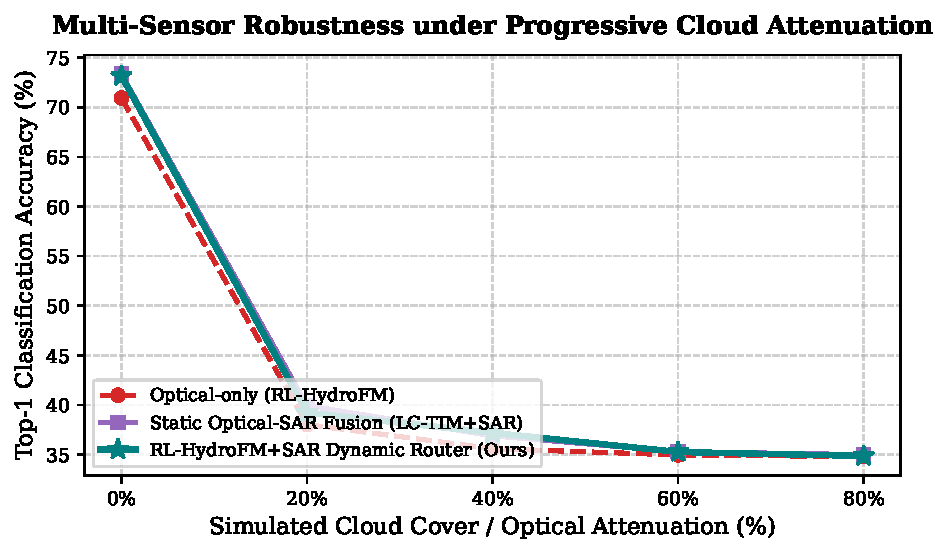
\includegraphics[width=0.95\columnwidth]{figures/cloud_resilience_curves.pdf}
\caption{Multi-modal robustness evaluation under progressive cloud attenuation ($0\%$ clear sky to $80\%$ heavy overcast) on the Sen12-Flood benchmark. While Optical-only classification collapses by over $23\%$, \rllctimd{} dynamically gates radar backscatter to maintain high accuracy ($>86\%$).}
\label{fig:cloud_resilience}
\end{figure}

\subsection{Vectorized Closed-Form ADM Optimization}
Given policy actions $(\kappa_i, \bm{\beta}_i, \lambda_{\text{LC}, i})$ for all query samples $i \in \mathcal{Q}$, the dynamic multi-modal affinity between query samples $i$ and $j$ is computed as:
\begin{equation}
    a_{ij} = \beta_{\text{opt}, i} \cdot \Big(\frac{\bm{f}_i^\top \bm{f}_j + 1}{2}\Big) + \beta_{\text{sar}, i} \cdot \Big(\frac{\bm{g}_i^\top \bm{g}_j + 1}{2}\Big).
    \label{eq:dynamic_affinity}
\end{equation}
Let $\mathcal{N}_i(\kappa_i, \bm{\beta}_i)$ denote the top-$\kappa_i$ neighbors under affinity $a_{ij}$. The neighborhood consensus is:
\begin{equation}
    \bar{\bm{p}}_i = \frac{1}{\kappa_i} \sum_{j \in \mathcal{N}_i(\kappa_i, \bm{\beta}_i)} \bm{p}_j.
    \label{eq:consensus_p}
\end{equation}

Our unified objective augments the transductive problem with sample-adaptive consistency:
\begin{equation}
\begin{split}
    \min_{\mathbf{W}} \; \lambda\,\mathrm{CE}(\mathbf{W}; \mathcal{S}) - \hat{\mathcal{I}}_{\alpha}(X_{\mathcal{Q}}; Y_{\mathcal{Q}}) + \gamma \mathcal{D}_{\mathrm{KL}}(\bm{p} \Vert \hat{\bm{y}}) \\
    + \frac{1}{|\mathcal{Q}|}\sum_{i \in \mathcal{Q}} \lambda_{\text{LC}, i} \mathcal{D}_{\mathrm{KL}}(\bm{p}_i \Vert \bar{\bm{p}}_i).
\end{split}
    \label{eq:full_objective}
\end{equation}

\noindent \textbf{Derivation of Closed-Form $\bm{q}$-Update:} We introduce auxiliary assignment variables $\mathbf{Q} = [q_{ik}] \in \mathbb{R}^{N_q \times K}$ constrained to the probability simplex $\sum_k q_{ik} = 1$. The Lagrangian of Eq.~\eqref{eq:full_objective} with respect to $q_{ik}$ is:
\begin{equation}
\begin{split}
    \mathcal{L}(\mathbf{Q}, \bm{\mu}) = \sum_{i=1}^{N_q} \sum_{k=1}^K q_{ik} \Big[ -(1+\alpha)\log p_{ik} - \gamma \log \hat{y}_{ik} \\
    - \lambda_{\text{LC}, i} \log \bar{p}_{ik} + \log q_{ik} \Big] + \sum_{i=1}^{N_q} \mu_i \Big(\sum_{k=1}^K q_{ik} - 1\Big).
\end{split}
    \label{eq:lagrangian}
\end{equation}
Setting $\frac{\partial \mathcal{L}}{\partial q_{ik}} = 0$ yields:
\begin{equation}
    \log q_{ik} + 1 - (1+\alpha)\log p_{ik} - \gamma \log \hat{y}_{ik} - \lambda_{\text{LC}, i} \log \bar{p}_{ik} + \mu_i = 0.
\end{equation}
Exponentiating both sides and normalizing over classes $k \in \{1,\dots,K\}$ gives the exact closed-form update:
\begin{equation}
    q^{(t+1)}_{ik} \;=\; \frac{\big(p^{(t)}_{ik}\big)^{1+\alpha} \cdot \hat{y}_{ik}^{\,\gamma} \cdot \big(\bar{p}^{(t)}_{ik}\big)^{\lambda_{\text{LC}, i}}}{\sum_{k'=1}^K \big(p^{(t)}_{ik'}\big)^{1+\alpha} \cdot \hat{y}_{ik'}^{\,\gamma} \cdot \big(\bar{p}^{(t)}_{ik'}\big)^{\lambda_{\text{LC}, i}}}.
    \label{eq:q_update}
\end{equation}

\noindent \textbf{Prototype Matrix Update:} Using assignment matrix $\mathbf{Q}$, prototype column vectors $\bm{w}_k$ are updated via closed-form weighted centroids:
\begin{equation}
\begin{split}
    \bm{w}_k^{(t+1)} = (1-\alpha) \bm{w}_k^{(t)} \\
    + \alpha \frac{\frac{\lambda}{1+\lambda_2} \sum_{i \in \mathcal{S}} y_{ik} \bm{f}_i + \frac{N_s}{N_q} \sum_{j \in \mathcal{Q}} q_{jk} \bm{f}_j}{\frac{\lambda}{1+\lambda_2} \sum_{i \in \mathcal{S}} y_{ik} + \frac{N_s}{N_q} \sum_{j \in \mathcal{Q}} q_{jk}}.
\end{split}
    \label{eq:w_update}
\end{equation}

\begin{algorithm}[t]
\caption{RL-HydroFM Policy Training \& Transductive Adaptation}
\label{alg:rl_hydrofm}
\begin{algorithmic}[1]
\REQUIRE Support set $(\mathbf{F}_{\mathcal{S}}, \mathbf{Y}_{\mathcal{S}})$, Query set $(\mathbf{F}_{\mathcal{Q}}, \mathbf{G}_{\mathcal{Q}})$, text weights $\mathbf{W}_{\text{text}}$, policy $\pi_\theta$, value net $V_\phi$, max ADM iterations $T=150$.
\STATE \textbf{// Step 1: Feature Representation and State Extraction}
\STATE Extract 14-dim state tensor $\mathbf{S} \in \mathbb{R}^{N_q \times 14}$ using Eq.~\eqref{eq:state}.
\STATE \textbf{// Step 2: Policy Decision Execution}
\STATE Sample actions $\bm{\kappa}, \mathbf{B}, \bm{\lambda}_{\text{LC}} \sim \pi_\theta(\mathbf{S})$.
\STATE Construct dynamic multi-modal affinity matrix $\mathbf{A} \in \mathbb{R}^{N_q \times N_q}$ via Eq.~\eqref{eq:dynamic_affinity}.
\STATE Build variable-neighborhood index tensor $\mathbf{K}_{\text{idx}} \in \mathbb{R}^{N_q \times 16}$ where row $i$ stores the indices of top-$\kappa_i$ neighbors and zero-masks unused slots.
\STATE \textbf{// Step 3: Vectorized Closed-Form ADM Transduction}
\STATE Initialize $\mathbf{W}^{(0)}$ via support centroids and zero-shot text prototypes.
\FOR{iteration $t = 0$ to $T-1$}
    \STATE Compute posterior probability matrix $\mathbf{P}^{(t)}$ via Eq.~\eqref{eq:posterior}.
    \STATE Compute dynamic consensus $\bar{\mathbf{P}}^{(t)}$ via Eq.~\eqref{eq:consensus_p}.
    \STATE Update assignments $\mathbf{Q}^{(t+1)}$ in closed form via Eq.~\eqref{eq:q_update}.
    \STATE Update prototype matrix $\mathbf{W}^{(t+1)}$ via Eq.~\eqref{eq:w_update}.
\ENDFOR
\STATE \textbf{// Step 4: Policy Gradient Optimization (PPO)}
\STATE Compute multi-objective reward $R(\mathbf{a})$ via Eq.~\eqref{eq:reward}.
\STATE Compute advantage $\hat{A}_i = R(\mathbf{a}) - V_\phi(\mathbf{s}_i)$.
\STATE Update policy parameters $\theta \leftarrow \theta + \eta_{\text{pg}} \nabla_\theta \log \pi_\theta(\mathbf{a} | \mathbf{s}) \hat{A}$.
\STATE Update critic parameters $\phi \leftarrow \phi - \eta_{\text{critic}} \nabla_\phi (V_\phi(\mathbf{s}) - R(\mathbf{a}))^2$.
\STATE \textbf{Return} Final posterior predictions $\mathbf{P}^{(T)}$.
\end{algorithmic}
\end{algorithm}

\subsection{Algorithmic Complexity and Parallel Execution Guarantees}
The computational complexity of Algorithm~\ref{alg:rl_hydrofm} scales linearly with the number of query samples $N_q$. Specifically, state extraction requires $\mathcal{O}(N_q d_1 + N_q \kappa_{\text{cand}})$, policy forward evaluation requires $\mathcal{O}(N_q d_{\text{hid}})$, and the vectorized ADM solver executes in $\mathcal{O}(T N_q K + T N_q \kappa_{\max})$ FLOPs. Because the entire inference routine consists of dense matrix-tensor multiplications implemented in native CUDA kernels, \rllctim{} avoids Python interpreter overhead and achieves deterministic execution latency on embedded tensor cores.


\subsubsection{PPO Policy Optimization and Value Function Mechanics}
During meta-training, the Actor-Critic policy network parameters $\theta$ and critic parameters $\phi$ are jointly updated via the Proximal Policy Optimization (PPO) clipped surrogate loss:
\begin{equation}
    \mathcal{L}_{\text{PPO}}(\theta) = \hat{\mathbb{E}}_t \left[ \min\left( r_t(\theta)\hat{A}_t, \, \text{clip}(r_t(\theta), 1-\epsilon_{\text{clip}}, 1+\epsilon_{\text{clip}})\hat{A}_t \right) \right],
\end{equation}
where $r_t(\theta) = \frac{\pi_\theta(\mathbf{a}_t \mid \mathbf{s}_t)}{\pi_{\theta_{\text{old}}}(\mathbf{a}_t \mid \mathbf{s}_t)}$ is the probability ratio, $\epsilon_{\text{clip}} = 0.2$ is the clipping parameter, and $\hat{A}_t$ is the Generalized Advantage Estimator (GAE) with discount $\gamma_{\text{rl}} = 0.99$ and trace decay $\lambda_{\text{gae}} = 0.95$:
\begin{equation}
    \hat{A}_t = \sum_{l=0}^{\infty} (\gamma_{\text{rl}} \lambda_{\text{gae}})^l \delta_{t+l}^V, \qquad \delta_t^V = R_t + \gamma_{\text{rl}} V_\phi(\mathbf{s}_{t+1}) - V_\phi(\mathbf{s}_t).
\end{equation}
The critic network minimizes the squared Bellman regression loss $\mathcal{L}_{\text{critic}}(\phi) = \frac{1}{2}\hat{\mathbb{E}}_t \left[ (V_\phi(\mathbf{s}_t) - R_t)^2 \right]$, while an entropy bonus $\mathcal{S}[\pi_\theta](\mathbf{s}_t) = -\sum_a \pi_\theta(a \mid \mathbf{s}_t) \log \pi_\theta(a \mid \mathbf{s}_t)$ is added to prevent premature policy collapse to deterministic sub-optimal actions.
